\documentclass[12pt,a4paper]{article}
\usepackage{geometry}
\usepackage{slashbox}
\geometry{
	a4paper,
	total={170mm,257mm},
	left=20mm,
	top=20mm,
}
\usepackage{graphicx}
\usepackage{pdfpages}

\usepackage{polski}
\usepackage[utf8]{inputenc}

\begin{document}
	
	\begin{titlepage}
		\newgeometry{top=5.5cm, bottom=3cm}
		
		\centering
		{\huge\bfseries Logika układów cyfrowych lab.\par}
		
		\vspace{0.5cm}
		Prowadzący: Antoni Sterna (E02-38m, wtorek 17:05) \\
	
		\vspace{1.1cm}
		{\Large sprawozdanie 2 - 2017.10.17\par}
		\vfill
		
		{\large\bfseries Jakub Dorda 235013\par}
		{\large\bfseries Marcin Kotas 235098\par}
		
		\vspace{1cm}
		\today \\ \LaTeX
		
		\restoregeometry
	\end{titlepage}

	
	\section{Wprowadzenie/cel ćwiczeń}
	
		Celem pierwszego zadania było stworzenie transkodera naturalnego kodu binarnego 3 bitowego wykonującego dla każdego przypadku operację dodawania +3. Kolejnym Zadaniem było wykonanie Subtraktora pełnego 1 bitowego. trudność w drugim zadaniu polegała na ograniczeniu implementacji tylko do dwuwejściowych bramek NAND. Obydwa układy zostały sprawdzone w symulatorze oraz przez wykonanie ich na zestawie prototypowym w czasie zajęć w laboratorium. 
	
	\section{Transkoder naturalnego kodu binarnego na kod +3}
		
		\subsection{Tabela prawdy i tablice Karnaugh:}
			
			\begin{table}[h]
				\begin{minipage}{.5\textwidth}
					\caption{Tabela Prawdy}
					\vspace{0.2cm}
					\centering
					\begin{tabular}{ccc|c|c|c|c}
						a&b&c&y\textsubscript{3}&y\textsubscript{2}&y\textsubscript{1}&y\textsubscript{0}\\\hline
						0&0&0&0&0&1&1\\
						0&0&1&0&1&0&0\\
						0&1&0&0&1&0&1\\
						0&1&1&0&1&1&0\\\hline
						1&0&0&0&1&1&1\\
						1&0&1&1&0&0&0\\
						1&1&0&1&0&0&1\\
						1&1&1&1&0&1&0\\
					\end{tabular}
					\vspace{1cm}
					\caption{Tablica Karnaugh dla y\textsubscript{3}}
					\vspace{0.2cm}
					\centering
					\begin{tabular}{c|c|c|c|c}
						\backslashbox{c}{ab}&00&01&11&10\\\hline
						0&0&0&1&0\\\hline
						1&0&0&1&1\\
					\end{tabular}
				\end{minipage}%
				\begin{minipage}{.5\textwidth}
					\caption{Tablica Karnaugh dla y\textsubscript{2}}
					\vspace{0.2cm}
					\centering
					\begin{tabular}{c|c|c|c|c}
						\backslashbox{c}{ab}&00&01&11&10\\\hline
						0&0&1&0&1\\\hline
						1&1&1&0&0\\
					\end{tabular}
					\vspace{0.4cm}
				 	\caption{Tablica Karnaugh dla y\textsubscript{1}}
				 	\vspace{0.2cm}
				 	\centering
				 	\begin{tabular}{c|c|c|c|c}
				 		\backslashbox{c}{ab}&00&01&11&10\\\hline
				 		0&1&0&0&1\\\hline
				 		1&0&1&1&0\\
				 	\end{tabular} 
			 		\vspace{0.4cm}
			 		\caption{Tablica Karnaugh dla y\textsubscript{0}}
			 		\vspace{0.2cm}
			 		\centering
			 		\begin{tabular}{c|c|c|c|c}
			 			\backslashbox{c}{ab}&00&01&11&10\\\hline
			 			0&1&1&1&1\\\hline
			 			1&0&0&0&0\\
			 		\end{tabular} 
				\end{minipage} 
			\end{table}
				
		\subsection{Minimalizacje:}
			
			\begin{minipage}{.5\textwidth}
				\begin{displaymath}
				y_3 = ab + ac = \overline{\overline{ab}\cdot\overline{ac}}
				\end{displaymath}
				\begin{displaymath}
				y_2 = a\bar{b}\bar{c} + \bar{a}b + \bar{a}c
				= \overline{\overline{a\bar{b}\bar{c}}\cdot\overline{\bar{a}b}\cdot\overline{\bar{a}c}}
				\end{displaymath}
			\end{minipage}%
			\begin{minipage}{.5\textwidth}
				\begin{displaymath}
				y_1 = bc + \bar{b}\bar{c}
				= \overline{\overline{bc}\cdot\overline{\bar{b}\bar{c}}}
				\end{displaymath}
				\begin{displaymath}
				y_0 = \bar{c}
				\end{displaymath}
			\end{minipage}
			
		\subsection{Użyte wzory:}
			\begin{equation}
			\overline{a\cdot b}=\bar{a}+\bar{b}
			\end{equation}
			\begin{equation}
			\overline{a+b}=\bar{a}\cdot\bar{b}
			\end{equation}
			
		\subsection{Schemat układu:}
		
		\vspace{0.5cm}
		\begin{center}
			\makebox[\textwidth]{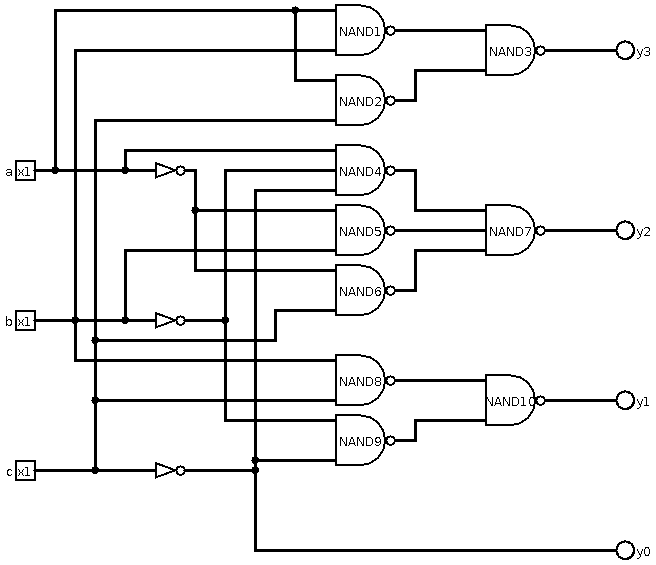
\includegraphics[width=\paperwidth - 80mm]{schem/circuit.png}}
			Schemat 1. Układ transkodera na bramkach NAND
		\end{center}
		
	\section{Subtraktor pełny 1 bitowy (na NAND 2 wejściowych)}
		
		\subsection{Tabela prawdy i tablice Karnaugh:}
			
			\begin{table}[h]
				\begin{minipage}{.5\textwidth}
					\caption{Tabela Prawdy}
					\vspace{0.2cm}
					\centering
					\begin{tabular}{ccc|c|c}
						A&B&C&D\textsubscript{i}&C\textsubscript{i+1}\\\hline
						0&0&0&0&0\\
						0&0&1&1&1\\
						0&1&0&1&1\\
						0&1&1&0&1\\\hline
						1&0&0&1&0\\
						1&0&1&0&0\\
						1&1&0&0&0\\
						1&1&1&1&1\\
					\end{tabular}
					\begin{displaymath}
					D_i = A_i \oplus B_i \oplus C_i
					\end{displaymath}
					\begin{displaymath}
					C_{i+1} = A_i < (B_i + C_i)
					\end{displaymath}
				\end{minipage}%
				\begin{minipage}{.5\textwidth}
					\caption{Tablica Karnaugh dla D\textsubscript{i}}
					\vspace{0.2cm}
					\centering
					\begin{tabular}{c|c|c|c|c}
						\backslashbox{C}{AB}&00&01&11&10\\\hline
						0&0&1&0&1\\\hline
						1&1&0&1&0\\
					\end{tabular}
					\vspace{0.4cm}
					\caption{Tablica Karnaugh dla C\textsubscript{i+1}}
					\vspace{0.2cm}
					\centering
					\begin{tabular}{c|c|c|c|c}
						\backslashbox{C}{AB}&00&01&11&10\\\hline
						0&0&1&0&0\\\hline
						1&1&1&1&0\\
					\end{tabular} 
				\end{minipage} 
			\end{table}
			
			\noindent
			$A_i$ - odjemna, $B_i$ - odjemnik, $C_i$ - pożyczka od poprzedniego bitu\\
			$D_i$ - bit różnicy/wynik, $C_{i+1}$ - bit pożyczki/przeniesienie
				
		\subsection{Minimalizacje:}
			
			\begin{displaymath}
				D_i = \bar{a}\bar{b}c + \bar{a}b\bar{c} + abc + a\bar{b}\bar{c}
				= \bar{a}(\bar{b}c+b\bar{c}) + a(bc + \bar{b}\bar{c})
				= \overline{\overline{\bar{a}(\bar{b}c+b\bar{c})}\cdot\overline{a(bc + \bar{b}\bar{c})}}
				= \overline{\overline{\bar{a}(\overline{\overline{\bar{b}c}\cdot\overline{b\bar{c}}})}
					\cdot\overline{a(\overline{\overline{bc} \cdot \overline{\bar{b}\bar{c}}})}}
			\end{displaymath}
			\begin{displaymath}
				C_{i+1} = \bar{a}b+\bar{a}c+bc
				= \bar{a}b+c(\bar{a}+b)
				= \overline{\overline{\bar{a}b}\cdot\overline{c(\bar{a}+b)}}
				= \overline{\overline{\bar{a}b}\cdot\overline{c(\overline{\bar{\bar{a}}\cdot\bar{b}})}}
				= \overline{\overline{\bar{a}b}\cdot\overline{c(\overline{a\cdot\bar{b}})}}
			\end{displaymath}
		
		\subsection{Użyte wzory:}
			\begin{equation}
			\overline{a\cdot b}=\bar{a}+\bar{b}
			\end{equation}
			\begin{equation}
			\overline{a+b}=\bar{a}\cdot\bar{b}
			\end{equation}
			
		\subsection{Schemat układu:}
		
		\vspace{0.5cm}
		\begin{center}
			\makebox[\textwidth]{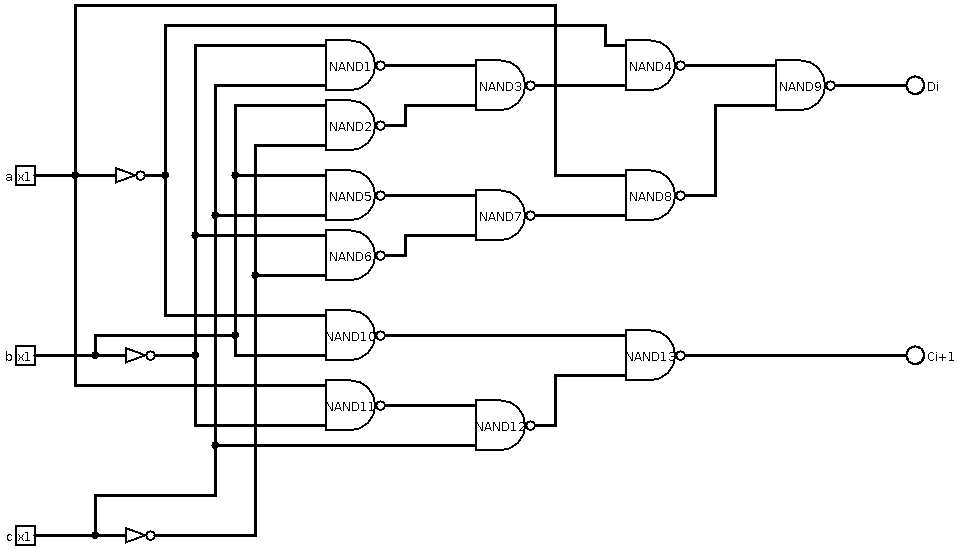
\includegraphics[width=\paperwidth - 40mm]{schem/circuit2.png}}
			Schemat 1. Układ subtraktora na dwuwejściowych bramkach NAND
		\end{center}

	\section{Wnioski/podsumowanie}
	
	W celu sprawdzenie poprawności działania należało przeprowadzić testy dla wszystkich możliwych kombinacji wejść w tym przypadku dla obu układów było to $2^3 = 8$. Obydwa układy działały poprawnie, aczkolwiek w przypadku pierwszego zadania możliwa była dalsza minimalizacja oraz użycie innych bramek w celu uproszczenia finalnego układu. 
	
\end{document}